\documentclass[11pt]{article}

\usepackage[T1]{fontenc}
\usepackage{lmodern}
\usepackage[margin=1in]{geometry}
\usepackage{amsmath,amssymb}
\usepackage{graphicx}
\usepackage{booktabs}
\usepackage{array}
\usepackage{xcolor}
\usepackage{tikz}
\usetikzlibrary{arrows.meta,positioning,fit,backgrounds,calc}
\usepackage{enumitem}
\usepackage{microtype}
\usepackage{caption}
\usepackage[numbers,sort&compress]{natbib}
\usepackage{authblk}
\usepackage[colorlinks=true,linkcolor=blue,citecolor=blue,urlcolor=blue]{hyperref}

\newcommand{\sysname}{MemoPilot~IQ}
\newcommand{\layername}{MemoPilot memory layer}

\hypersetup{
  pdftitle={MemoPilot IQ: Auditable Lifecycle Governance for Persistent Agent Memory},
  pdfauthor={Mahar Muavia, Muhammad Imran Shah, Tayyaba Shehzad},
  pdfsubject={Persistent memory governance for language-model agents},
  pdfkeywords={agent memory, lifecycle governance, retrieval, auditability}
}

\title{\textbf{\sysname{}: Auditable Lifecycle Governance\\
for Persistent Agent Memory}}

\author[1]{Mahar Muavia\thanks{Corresponding author: \texttt{contact@inventacore.org}}}
\author[1]{Muhammad Imran Shah}
\author[1]{Tayyaba Shehzad}
\affil[1]{InventaCore AI \quad \url{https://inventacore.org}}
\date{Technical report, July 2026}

\begin{document}
\maketitle

\begin{abstract}
Persistent assistants need more than a store of old messages. They need rules
for deciding which information is current, which information has expired, and
which records may enter a limited model context. We describe \sysname{}, an
open-source assistant whose memory layer represents conversation-derived facts
as typed records with explicit lifecycle states. Retrieval combines dense and
lexical signals with a transparent ranking function. A context builder then
selects records under a hard 2,500-token memory budget and a default top-eight
relevance window, and a per-answer trace records every inclusion and exclusion
decision. Inactive records are excluded from normal retrieval while lifecycle
decisions remain auditable. In a deterministic 24-scenario diagnostic, the
current implementation places the required memory in context for 21 of 22
eligible scenarios, injects no stale record across 24 scenarios, and uses 31\%
fewer estimated historical-context tokens than replaying the setup messages.
Removing lifecycle exclusion increases the stale-injection rate from 0.00 to
0.33; changing the ranking weights or priority ordering does not change the
measured outcomes on this suite. The latter result limits, rather than
strengthens, the claim: the diagnostic validates lifecycle handling but is too
small to establish that the hand-set ranking weights are optimal. We release
the implementation, scenarios, trace format, and raw evaluation artifacts.
\end{abstract}

\section{Introduction}
\label{sec:intro}

A language-model assistant can appear stateful while a conversation is open,
but continuity usually depends on replaying messages inside a finite context
window. Across sessions, a developer must restate project choices, constraints,
deadlines, and preferences. Simply retaining every message creates a different
failure: old decisions remain available after they have been replaced.

Consider a project that begins with React and Vite and later moves to Next.js.
Both statements are relevant to a query about the frontend. A similarity search
can retrieve either one, even though only the later decision is valid. The
problem is therefore not just storage or nearest-neighbor search. The system
must represent the relationship between the two statements and prevent the old
one from entering the answer context.

This report treats persistent memory as a governance problem with four parts:

\begin{enumerate}[leftmargin=1.5em,itemsep=2pt]
  \item represent retained information as typed, inspectable records rather
  than an undifferentiated transcript;
  \item model expiry, archival, supersession, and deletion as explicit state
  transitions;
  \item assemble a small context under a hard budget while preserving a record
  of what was considered; and
  \item keep users able to inspect, edit, export, and erase memory.
\end{enumerate}

\sysname{} implements these choices in a provider-independent memory layer. In
online mode, Qwen supplies structured extraction, embeddings, and answer
generation. In deterministic offline mode, test doubles exercise the same
storage, lifecycle, retrieval, budgeting, and trace paths without credentials.
The evaluation in this report is intentionally limited to the latter mechanism
path. It does not present the offline answer generator as model evidence.

The contributions are practical rather than claims of state of the art:

\begin{itemize}[leftmargin=1.5em,itemsep=2pt]
  \item a typed memory record and auditable lifecycle with directed
  supersession links;
  \item hybrid retrieval, named ranking components, and strict context
  budgeting with a per-answer decision trace;
  \item explicit boundaries for untrusted stored text, secret redaction, and
  user memory controls; and
  \item a versioned diagnostic and ablation whose raw counts are generated from
  the same code shipped with the report.
\end{itemize}

\section{Related Work and Naming}
\label{sec:related}

Long-term memory for agents spans unstructured streams, hierarchical memory,
structured records, and temporal or graph-based stores; recent surveys provide
broader taxonomies~\citep{zhang2024survey,luo2026survey}. Generative Agents
rank a memory stream using relevance, recency, and importance and periodically
derive reflections~\citep{park2023generative}. MemGPT treats context management
as paging between limited in-context memory and external storage
~\citep{packer2023memgpt}. MemoryBank applies time-dependent memory strength
~\citep{zhong2024memorybank}, while A-Mem organizes linked notes that evolve as
new information arrives~\citep{xu2025amem}.

Production-oriented systems also perform memory extraction and update. Mem0
maintains selected facts in vector and optional graph stores
~\citep{chhikara2025mem0}. Zep represents changing information in a temporal
knowledge graph~\citep{rasmussen2025zep}. Empirical work shows why update and
deletion policy matters: replaying a similar but poor prior experience can
propagate errors into future behavior~\citep{xiong2026memory}. Preference-aware
updates address a related problem in long-running conversations
~\citep{sun2026preference}.

Two published systems use operating-system language for memory management.
MemoryOS uses hierarchical short-, mid-, and long-term stores
~\citep{kang2025memoryos}; MemOS proposes a broader resource abstraction across
plaintext, activation, and parameter memory~\citep{li2025memos}. The repository
for \sysname{} historically called its internal package ``MemoryOS.'' To avoid
confusing that implementation label with prior work, this report uses the term
\emph{MemoPilot memory layer} and makes no claim to the MemoryOS name.

LoCoMo provides a shared benchmark for long-conversation memory and includes
questions that require temporal, multi-hop, and open-domain reasoning
~\citep{maharana2024locomo}. Later work shows that factual string matching does
not cover implicit constraints or cognitive memory~\citep{li2026locomoplus}.
For that reason, the internal diagnostic reported here is treated as a narrow
engineering test. A complete, identically graded external comparison remains
future work.

\section{System Boundary and Threat Model}
\label{sec:threat}

The memory layer receives a user identifier, an optional project identifier, a
session identifier, and a message. It returns stored-memory actions and, when
answering, a bounded context plus a trace. Storage queries are scoped by user
and project. API-key middleware and rate limiting protect deployed endpoints,
but the memory layer itself does not establish user identity; a deployment must
bind those identifiers to authenticated principals.

Stored text is treated as untrusted data. The system prompt instructs the answer
model not to follow tool requests, safety overrides, or secret-exfiltration
instructions found in memory. Pattern-based detectors redact common API keys,
tokens, passwords, private-key blocks, and credential assignments before
persistence. This reduces accidental retention but is not a data-loss
prevention system and cannot detect every secret format.

Privacy labels are ranking metadata, not access control. A sensitive record
receives a score penalty, but authorization must still be enforced by the
application and storage layer. The evaluation does not establish resistance to
prompt injection, tenant-isolation attacks, or extraction of memorized text.

\section{Architecture}
\label{sec:architecture}

\sysname{} is a client/server application. A React/Vite frontend calls a
FastAPI backend. The memory layer owns extraction, persistence, retrieval,
ranking, lifecycle transitions, context assembly, and trace generation.
Figure~\ref{fig:arch} shows the request path.

% ---------------------------------------------------------------------------
% MemoPilot IQ / MemoryOS architecture figure (TikZ).
% Requires in the preamble:
%   \usepackage{tikz}
%   \usetikzlibrary{arrows.meta,positioning,fit,backgrounds,calc}
% Use with % ---------------------------------------------------------------------------
% MemoPilot IQ / MemoryOS architecture figure (TikZ).
% Requires in the preamble:
%   \usepackage{tikz}
%   \usetikzlibrary{arrows.meta,positioning,fit,backgrounds,calc}
% Use with % ---------------------------------------------------------------------------
% MemoPilot IQ / MemoryOS architecture figure (TikZ).
% Requires in the preamble:
%   \usepackage{tikz}
%   \usetikzlibrary{arrows.meta,positioning,fit,backgrounds,calc}
% Use with \input{figure_architecture} inside the document body.
% ---------------------------------------------------------------------------
\begin{figure*}[t]
\centering
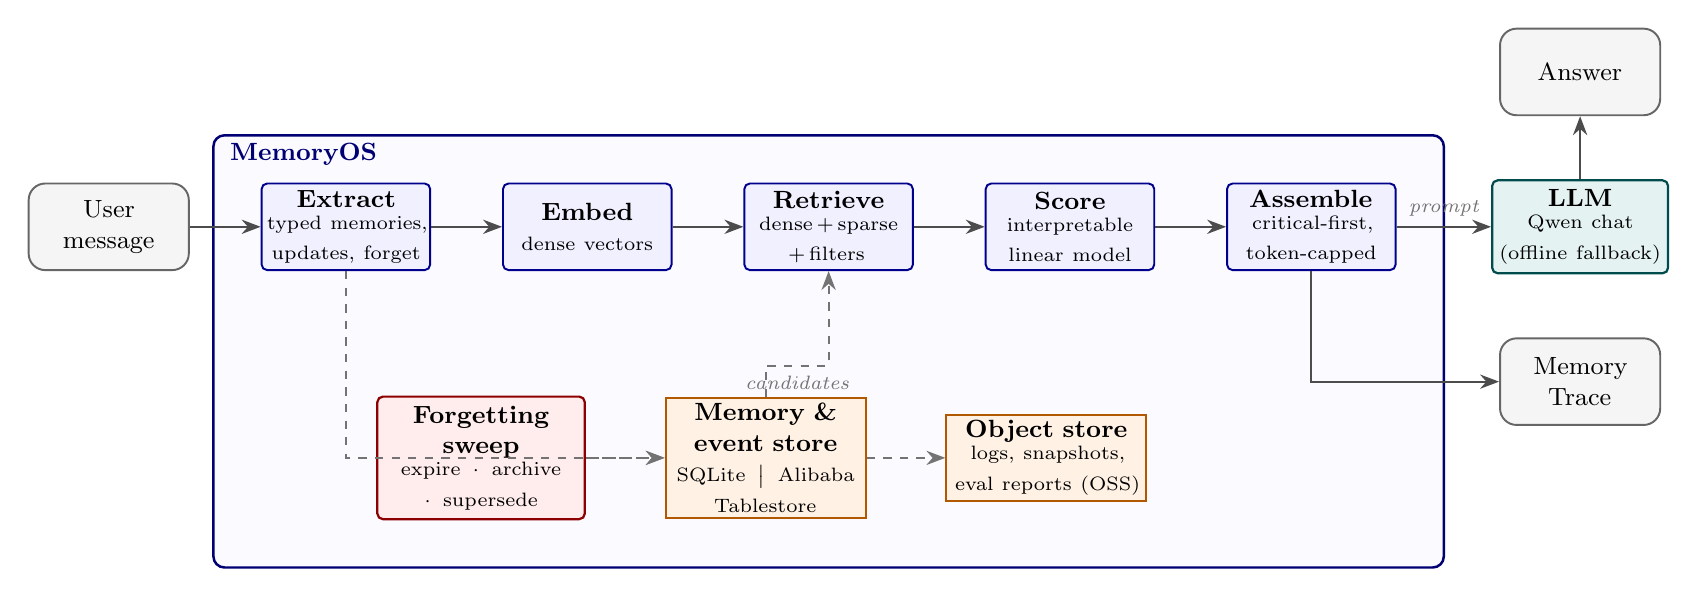
\begin{tikzpicture}[
  font=\small,
  node distance=6mm and 9mm,
  >={Stealth[length=2.4mm]},
  stage/.style={
    rectangle, rounded corners=2pt, draw=blue!55!black, line width=0.7pt,
    fill=blue!6, minimum height=11mm, text width=20mm, align=center,
    inner sep=2pt},
  edge/.style={->, line width=0.8pt, draw=black!70},
  dedge/.style={->, line width=0.7pt, draw=black!55, dashed},
  io/.style={
    rectangle, rounded corners=6pt, draw=black!60, line width=0.7pt,
    fill=black!4, minimum height=11mm, text width=18mm, align=center},
  llm/.style={
    rectangle, rounded corners=2pt, draw=teal!60!black, line width=0.8pt,
    fill=teal!10, minimum height=11mm, text width=20mm, align=center},
  store/.style={
    rectangle, draw=orange!70!black, line width=0.7pt, fill=orange!10,
    minimum height=10mm, text width=24mm, align=center, inner sep=2pt},
  forget/.style={
    rectangle, rounded corners=2pt, draw=red!55!black, line width=0.8pt,
    fill=red!7, minimum height=10mm, text width=24mm, align=center},
  lbl/.style={font=\scriptsize\itshape, text=black!55},
]

% ---- Input ----
\node[io] (user) {User\\message};

% ---- MemoryOS pipeline (left to right) ----
\node[stage, right=of user] (extract) {\textbf{Extract}\\\scriptsize typed memories,\\updates, forget};
\node[stage, right=of extract] (embed) {\textbf{Embed}\\\scriptsize dense vectors};
\node[stage, right=of embed] (retrieve) {\textbf{Retrieve}\\\scriptsize dense\,+\,sparse\\+\,filters};
\node[stage, right=of retrieve] (score) {\textbf{Score}\\\scriptsize interpretable\\linear model};
\node[stage, right=of score] (budget) {\textbf{Assemble}\\\scriptsize critical-first,\\token-capped};

% ---- LLM + outputs (far right, stacked) ----
\node[llm, right=12mm of budget] (llm) {\textbf{LLM}\\\scriptsize Qwen chat\\(offline fallback)};
\node[io, above=8mm of llm] (answer) {Answer};
\node[io, below=8mm of llm] (trace) {Memory\\Trace};

% ---- Pipeline edges ----
\draw[edge] (user) -- (extract);
\draw[edge] (extract) -- (embed);
\draw[edge] (embed) -- (retrieve);
\draw[edge] (retrieve) -- (score);
\draw[edge] (score) -- (budget);
\draw[edge] (budget) -- node[lbl, above]{prompt} (llm);
\draw[edge] (llm) -- (answer);
\draw[edge] (budget.south) |- (trace.west);

% ---- Storage layer (bottom) ----
\node[store, below=16mm of retrieve, xshift=-8mm] (db)
  {\textbf{Memory \& event store}\\\scriptsize SQLite \,$\big|$\, Alibaba Tablestore};
\node[store, right=10mm of db] (oss)
  {\textbf{Object store}\\\scriptsize logs, snapshots,\\eval reports (OSS)};

% ---- Forgetting engine ----
\node[forget, left=10mm of db] (forget)
  {\textbf{Forgetting sweep}\\\scriptsize expire \,$\cdot$\, archive\\$\cdot$\, supersede};

% ---- Storage edges ----
\draw[dedge] (extract.south) |- (db.west);
\draw[dedge] (db.north) -- ++(0,4mm) -| (retrieve.south)
  node[lbl, pos=0.25, below]{candidates};
\draw[dedge] (forget) -- (db);
\draw[dedge] (db) -- (oss);

% ---- MemoryOS grouping box ----
\begin{scope}[on background layer]
  \node[draw=blue!45!black, line width=0.9pt, rounded corners=4pt,
        fill=blue!2, inner sep=6mm,
        fit=(extract)(budget)(db)(oss)(forget)] (osbox) {};
  \node[anchor=north west, font=\small\bfseries, text=blue!45!black]
        at (osbox.north west) {\;MemoryOS};
\end{scope}

\end{tikzpicture}
\caption{Architecture and request lifecycle of \osname{}. A user message is
converted into \emph{typed} memories (Extract), embedded, and retrieved with a
hybrid dense\,+\,sparse signal under structured filters; candidates are ranked by
the interpretable linear score (Eq.~\ref{eq:score}) and assembled into the prompt
under a strict token budget that always injects critical/pinned memories. The LLM
produces the answer; a complete \emph{Memory Trace} records every inclusion and
skip decision. A periodic \emph{forgetting sweep} expires, archives, and
supersedes records out-of-band through auditable state transitions. The same
pipeline runs offline (SQLite, deterministic fallback) and in the cloud
(Tablestore\,/\,OSS, Qwen).}
\label{fig:arch}
\end{figure*}
 inside the document body.
% ---------------------------------------------------------------------------
\begin{figure*}[t]
\centering
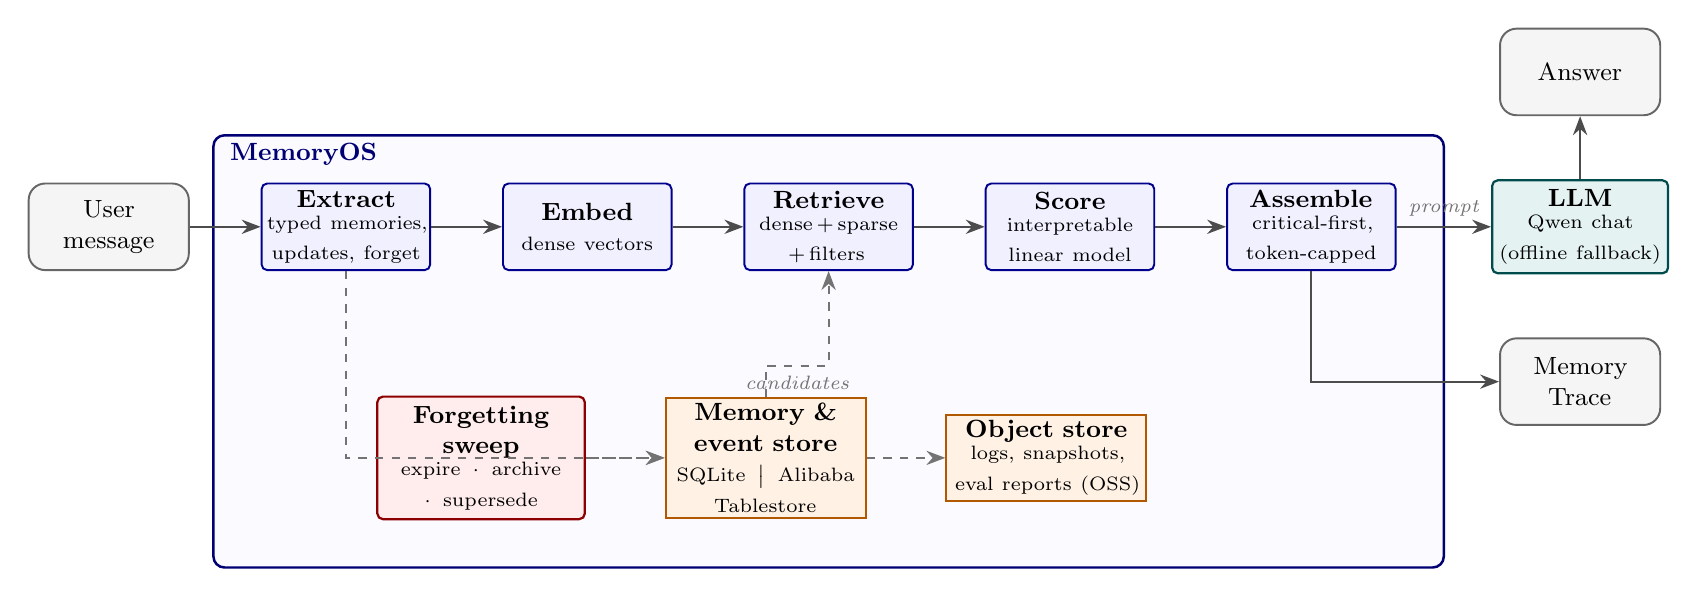
\begin{tikzpicture}[
  font=\small,
  node distance=6mm and 9mm,
  >={Stealth[length=2.4mm]},
  stage/.style={
    rectangle, rounded corners=2pt, draw=blue!55!black, line width=0.7pt,
    fill=blue!6, minimum height=11mm, text width=20mm, align=center,
    inner sep=2pt},
  edge/.style={->, line width=0.8pt, draw=black!70},
  dedge/.style={->, line width=0.7pt, draw=black!55, dashed},
  io/.style={
    rectangle, rounded corners=6pt, draw=black!60, line width=0.7pt,
    fill=black!4, minimum height=11mm, text width=18mm, align=center},
  llm/.style={
    rectangle, rounded corners=2pt, draw=teal!60!black, line width=0.8pt,
    fill=teal!10, minimum height=11mm, text width=20mm, align=center},
  store/.style={
    rectangle, draw=orange!70!black, line width=0.7pt, fill=orange!10,
    minimum height=10mm, text width=24mm, align=center, inner sep=2pt},
  forget/.style={
    rectangle, rounded corners=2pt, draw=red!55!black, line width=0.8pt,
    fill=red!7, minimum height=10mm, text width=24mm, align=center},
  lbl/.style={font=\scriptsize\itshape, text=black!55},
]

% ---- Input ----
\node[io] (user) {User\\message};

% ---- MemoryOS pipeline (left to right) ----
\node[stage, right=of user] (extract) {\textbf{Extract}\\\scriptsize typed memories,\\updates, forget};
\node[stage, right=of extract] (embed) {\textbf{Embed}\\\scriptsize dense vectors};
\node[stage, right=of embed] (retrieve) {\textbf{Retrieve}\\\scriptsize dense\,+\,sparse\\+\,filters};
\node[stage, right=of retrieve] (score) {\textbf{Score}\\\scriptsize interpretable\\linear model};
\node[stage, right=of score] (budget) {\textbf{Assemble}\\\scriptsize critical-first,\\token-capped};

% ---- LLM + outputs (far right, stacked) ----
\node[llm, right=12mm of budget] (llm) {\textbf{LLM}\\\scriptsize Qwen chat\\(offline fallback)};
\node[io, above=8mm of llm] (answer) {Answer};
\node[io, below=8mm of llm] (trace) {Memory\\Trace};

% ---- Pipeline edges ----
\draw[edge] (user) -- (extract);
\draw[edge] (extract) -- (embed);
\draw[edge] (embed) -- (retrieve);
\draw[edge] (retrieve) -- (score);
\draw[edge] (score) -- (budget);
\draw[edge] (budget) -- node[lbl, above]{prompt} (llm);
\draw[edge] (llm) -- (answer);
\draw[edge] (budget.south) |- (trace.west);

% ---- Storage layer (bottom) ----
\node[store, below=16mm of retrieve, xshift=-8mm] (db)
  {\textbf{Memory \& event store}\\\scriptsize SQLite \,$\big|$\, Alibaba Tablestore};
\node[store, right=10mm of db] (oss)
  {\textbf{Object store}\\\scriptsize logs, snapshots,\\eval reports (OSS)};

% ---- Forgetting engine ----
\node[forget, left=10mm of db] (forget)
  {\textbf{Forgetting sweep}\\\scriptsize expire \,$\cdot$\, archive\\$\cdot$\, supersede};

% ---- Storage edges ----
\draw[dedge] (extract.south) |- (db.west);
\draw[dedge] (db.north) -- ++(0,4mm) -| (retrieve.south)
  node[lbl, pos=0.25, below]{candidates};
\draw[dedge] (forget) -- (db);
\draw[dedge] (db) -- (oss);

% ---- MemoryOS grouping box ----
\begin{scope}[on background layer]
  \node[draw=blue!45!black, line width=0.9pt, rounded corners=4pt,
        fill=blue!2, inner sep=6mm,
        fit=(extract)(budget)(db)(oss)(forget)] (osbox) {};
  \node[anchor=north west, font=\small\bfseries, text=blue!45!black]
        at (osbox.north west) {\;MemoryOS};
\end{scope}

\end{tikzpicture}
\caption{Architecture and request lifecycle of \osname{}. A user message is
converted into \emph{typed} memories (Extract), embedded, and retrieved with a
hybrid dense\,+\,sparse signal under structured filters; candidates are ranked by
the interpretable linear score (Eq.~\ref{eq:score}) and assembled into the prompt
under a strict token budget that always injects critical/pinned memories. The LLM
produces the answer; a complete \emph{Memory Trace} records every inclusion and
skip decision. A periodic \emph{forgetting sweep} expires, archives, and
supersedes records out-of-band through auditable state transitions. The same
pipeline runs offline (SQLite, deterministic fallback) and in the cloud
(Tablestore\,/\,OSS, Qwen).}
\label{fig:arch}
\end{figure*}
 inside the document body.
% ---------------------------------------------------------------------------
\begin{figure*}[t]
\centering
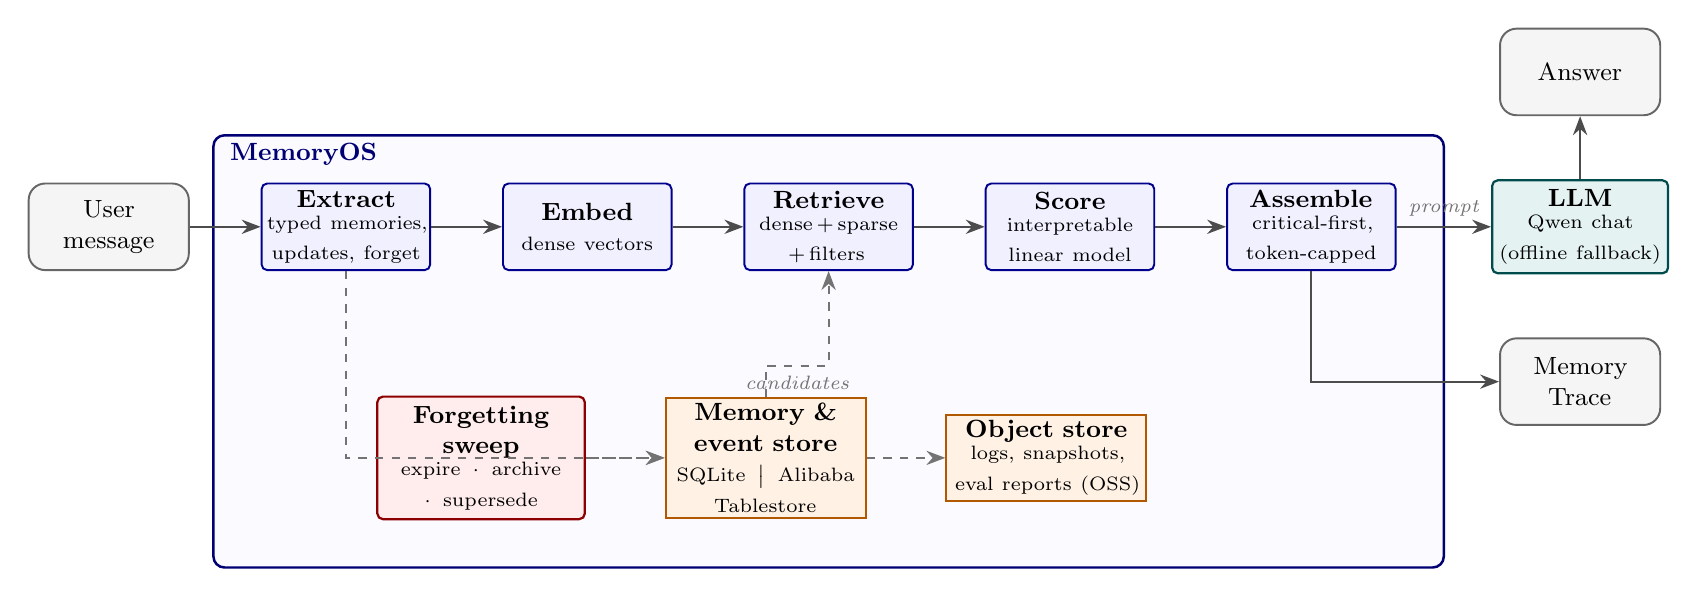
\begin{tikzpicture}[
  font=\small,
  node distance=6mm and 9mm,
  >={Stealth[length=2.4mm]},
  stage/.style={
    rectangle, rounded corners=2pt, draw=blue!55!black, line width=0.7pt,
    fill=blue!6, minimum height=11mm, text width=20mm, align=center,
    inner sep=2pt},
  edge/.style={->, line width=0.8pt, draw=black!70},
  dedge/.style={->, line width=0.7pt, draw=black!55, dashed},
  io/.style={
    rectangle, rounded corners=6pt, draw=black!60, line width=0.7pt,
    fill=black!4, minimum height=11mm, text width=18mm, align=center},
  llm/.style={
    rectangle, rounded corners=2pt, draw=teal!60!black, line width=0.8pt,
    fill=teal!10, minimum height=11mm, text width=20mm, align=center},
  store/.style={
    rectangle, draw=orange!70!black, line width=0.7pt, fill=orange!10,
    minimum height=10mm, text width=24mm, align=center, inner sep=2pt},
  forget/.style={
    rectangle, rounded corners=2pt, draw=red!55!black, line width=0.8pt,
    fill=red!7, minimum height=10mm, text width=24mm, align=center},
  lbl/.style={font=\scriptsize\itshape, text=black!55},
]

% ---- Input ----
\node[io] (user) {User\\message};

% ---- MemoryOS pipeline (left to right) ----
\node[stage, right=of user] (extract) {\textbf{Extract}\\\scriptsize typed memories,\\updates, forget};
\node[stage, right=of extract] (embed) {\textbf{Embed}\\\scriptsize dense vectors};
\node[stage, right=of embed] (retrieve) {\textbf{Retrieve}\\\scriptsize dense\,+\,sparse\\+\,filters};
\node[stage, right=of retrieve] (score) {\textbf{Score}\\\scriptsize interpretable\\linear model};
\node[stage, right=of score] (budget) {\textbf{Assemble}\\\scriptsize critical-first,\\token-capped};

% ---- LLM + outputs (far right, stacked) ----
\node[llm, right=12mm of budget] (llm) {\textbf{LLM}\\\scriptsize Qwen chat\\(offline fallback)};
\node[io, above=8mm of llm] (answer) {Answer};
\node[io, below=8mm of llm] (trace) {Memory\\Trace};

% ---- Pipeline edges ----
\draw[edge] (user) -- (extract);
\draw[edge] (extract) -- (embed);
\draw[edge] (embed) -- (retrieve);
\draw[edge] (retrieve) -- (score);
\draw[edge] (score) -- (budget);
\draw[edge] (budget) -- node[lbl, above]{prompt} (llm);
\draw[edge] (llm) -- (answer);
\draw[edge] (budget.south) |- (trace.west);

% ---- Storage layer (bottom) ----
\node[store, below=16mm of retrieve, xshift=-8mm] (db)
  {\textbf{Memory \& event store}\\\scriptsize SQLite \,$\big|$\, Alibaba Tablestore};
\node[store, right=10mm of db] (oss)
  {\textbf{Object store}\\\scriptsize logs, snapshots,\\eval reports (OSS)};

% ---- Forgetting engine ----
\node[forget, left=10mm of db] (forget)
  {\textbf{Forgetting sweep}\\\scriptsize expire \,$\cdot$\, archive\\$\cdot$\, supersede};

% ---- Storage edges ----
\draw[dedge] (extract.south) |- (db.west);
\draw[dedge] (db.north) -- ++(0,4mm) -| (retrieve.south)
  node[lbl, pos=0.25, below]{candidates};
\draw[dedge] (forget) -- (db);
\draw[dedge] (db) -- (oss);

% ---- MemoryOS grouping box ----
\begin{scope}[on background layer]
  \node[draw=blue!45!black, line width=0.9pt, rounded corners=4pt,
        fill=blue!2, inner sep=6mm,
        fit=(extract)(budget)(db)(oss)(forget)] (osbox) {};
  \node[anchor=north west, font=\small\bfseries, text=blue!45!black]
        at (osbox.north west) {\;MemoryOS};
\end{scope}

\end{tikzpicture}
\caption{Architecture and request lifecycle of \osname{}. A user message is
converted into \emph{typed} memories (Extract), embedded, and retrieved with a
hybrid dense\,+\,sparse signal under structured filters; candidates are ranked by
the interpretable linear score (Eq.~\ref{eq:score}) and assembled into the prompt
under a strict token budget that always injects critical/pinned memories. The LLM
produces the answer; a complete \emph{Memory Trace} records every inclusion and
skip decision. A periodic \emph{forgetting sweep} expires, archives, and
supersedes records out-of-band through auditable state transitions. The same
pipeline runs offline (SQLite, deterministic fallback) and in the cloud
(Tablestore\,/\,OSS, Qwen).}
\label{fig:arch}
\end{figure*}


The interfaces have two implementations. Local mode stores metadata and
embedding vectors in SQLite and uses deterministic extraction, embedding, and
answer fallbacks. Cloud mode connects the same interfaces to Qwen-compatible
chat and embedding endpoints, Alibaba Cloud Tablestore, and object storage. The
active provider and store are exposed by the health endpoint. Cloud adapters
are implemented, but this report does not claim a completed public deployment
or report cloud-model results.

\section{Memory Representation and Lifecycle}
\label{sec:schema}

The atomic unit is a \texttt{MemoryRecord}. Table~\ref{tab:fields} lists the
fields that affect governance.

\begin{table}[tbp]
\centering
\small
\caption{Selected fields of a \texttt{MemoryRecord}.}
\label{tab:fields}
\begin{tabular}{@{}lp{0.66\linewidth}@{}}
\toprule
\textbf{Field} & \textbf{Role} \\
\midrule
\texttt{type} & One of 12 categories: preference, project, decision, mistake,
constraint, deadline, learning goal, task, critical, temporary, outdated, or
deleted by user. \\
\texttt{status} & Active, pinned, archived, expired, superseded, or deleted. \\
\texttt{importance}, \texttt{confidence} & Bounded extraction metadata in
$[0,1]$. \\
\texttt{privacy\_level} & Public, private, or sensitive ranking metadata. \\
\texttt{expires\_at} & Optional expiry for temporary or dated records. \\
\texttt{supersedes}, \texttt{superseded\_by} & Directed links between an old
record and its replacement. \\
\texttt{usage\_count}, timestamps & Signals used for ranking and audit. \\
\bottomrule
\end{tabular}
\end{table}

\paragraph{Extraction.}
When a model provider is configured, a JSON-only ``Memory Editor'' proposes new
records, updates, and forget actions. Model output is not trusted: types and
privacy values are parsed against enums, importance and confidence are clamped,
content and tags have length limits, and secret redaction runs again before a
record is written. Offline mode uses a deterministic extractor for tests.

\paragraph{Supersession.}
The extractor compares a new record with active records in the same user and
project scope. Topic-specific replacement rules and structured model actions
can mark an older record \texttt{superseded} and link it to the replacement.
The old record remains visible in the timeline but normal retrieval excludes
it. This preserves the sequence of decisions without allowing the older choice
to compete in answer context.

\paragraph{Expiry and archival.}
A sweep runs before retrieval. A record whose \texttt{expires\_at} has passed
becomes \texttt{expired}. An active, non-critical record is archived when it is
unused, older than 30 days, and has importance below 0.35. Deletion is a
separate user action. Figure~\ref{fig:lifecycle} summarizes these transitions.

The delete endpoint defaults to a soft deletion that retains the record for
audit. A hard deletion removes the memory row, but the current event log retains
an audit entry. The implementation therefore does not claim cryptographic
erasure or deletion from storage-layer backups.

% ---------------------------------------------------------------------------
% Memory lifecycle state machine (TikZ). Compact wide layout.
% Requires: \usepackage{tikz,graphicx}; libraries arrows.meta, positioning,
% fit, backgrounds.
% ---------------------------------------------------------------------------
\begin{figure}[tbp]
\centering
\resizebox{0.95\linewidth}{!}{%
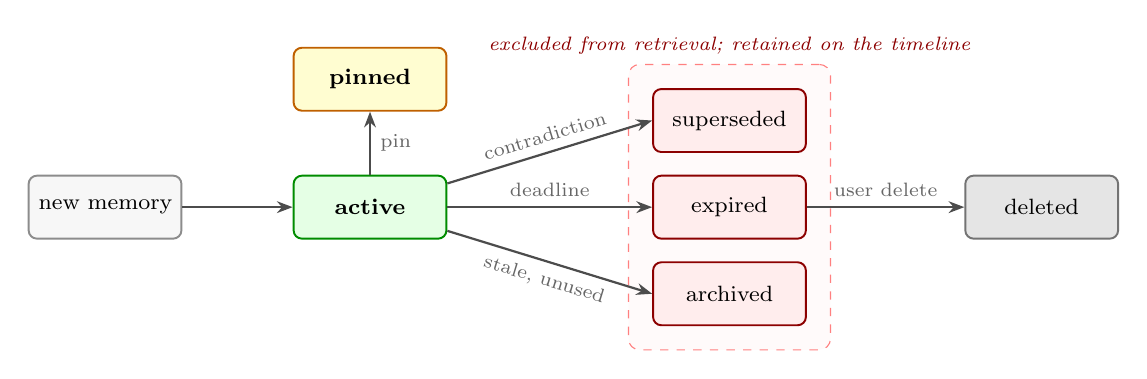
\begin{tikzpicture}[
  font=\footnotesize,
  >={Stealth[length=2mm]},
  st/.style={rounded corners=3pt, draw=black!60, line width=0.7pt,
    minimum height=8mm, text width=18mm, align=center, inner sep=2pt},
  active/.style={st, draw=green!55!black, fill=green!10},
  pinned/.style={st, draw=orange!75!black, fill=yellow!18},
  excl/.style={st, draw=red!55!black, fill=red!7},
  del/.style={st, draw=black!55, fill=black!10},
  e/.style={->, line width=0.8pt, draw=black!70},
  lbl/.style={font=\scriptsize, text=black!60},
]
\node[active] (active) {\textbf{active}};
\node[pinned, above=8mm of active] (pinned) {\textbf{pinned}};
\node[st, draw=black!45, fill=black!3, left=14mm of active] (new) {new memory};

\node[excl, right=26mm of active, yshift=11mm] (superseded) {superseded};
\node[excl, right=26mm of active] (expired) {expired};
\node[excl, right=26mm of active, yshift=-11mm] (archived) {archived};
\node[del, right=20mm of expired] (deleted) {deleted};

\draw[e] (new) -- (active);
\draw[e] (active.north) -- node[lbl, right]{pin} (pinned.south);
\draw[e] (active) -- node[lbl, above, sloped]{contradiction} (superseded.west);
\draw[e] (active) -- node[lbl, above]{deadline} (expired.west);
\draw[e] (active) -- node[lbl, below, sloped]{stale, unused} (archived.west);
\draw[e] (expired) -- node[lbl, above]{user delete} (deleted);

\begin{scope}[on background layer]
  \node[draw=red!50, dashed, rounded corners=4pt, fill=red!2, inner sep=3mm,
        fit=(superseded)(archived)] (exclbox) {};
  \node[anchor=south, font=\scriptsize\itshape, text=red!55!black]
        at (exclbox.north) {excluded from retrieval; retained on the timeline};
\end{scope}
\end{tikzpicture}%
}
\caption{The \texttt{MemoryRecord} lifecycle as an auditable state machine. A
new memory is born \texttt{active} (or \texttt{pinned} on user request). It is
\texttt{superseded} by a contradicting decision, \texttt{expired} when its
deadline passes, or \texttt{archived} when stale and unused; only an explicit
user action \texttt{deletes} it. Crucially, the \texttt{superseded},
\texttt{expired}, and \texttt{archived} states are excluded from retrieval yet
retained on the timeline, so the agent never reasons from invalid memory while
the history stays complete and reversible.}
\label{fig:lifecycle}
\end{figure}


\section{Retrieval and Ranking}
\label{sec:retrieval}

Retrieval first excludes archived, expired, superseded, and deleted records.
For each remaining record $m$ and query $q$, the implementation computes dense
cosine similarity $d(m,q)\in[0,1]$ and lexical overlap

\begin{equation}
k(m,q) = \frac{|T(q)\cap T(m)|}{|T(q)|},
\end{equation}

where $T(\cdot)$ is the set of lowercase alphanumeric tokens and $T(m)$ also
includes tags. The hybrid relevance signal is

\begin{equation}
r(m,q) = \max\left(d(m,q),\frac{d(m,q)+k(m,q)}{2}\right).
\end{equation}

The ranking score combines relevance with record metadata:

\begin{equation}
\label{eq:score}
\begin{aligned}
S(m,q) ={}& 0.40r + 0.20I + 0.15R + 0.10C + 0.10U \\
          & + 0.15P + 0.20K - 0.30O - 0.25V - 0.50X.
\end{aligned}
\end{equation}

$I$ is importance, $C$ confidence, $P$ project match, and $K$ a critical or
pinned indicator. $O$, $V$, and $X$ penalize outdated, private/sensitive, and
superseded/expired/deleted records. Recency uses
$R=\exp(-\Delta t/14)$ with $\Delta t$ in days; 14 days is the exponential
time constant, not the half-life. Usage is
$U=1-(1+\ln(1+u))^{-1}$ for usage count $u$.

The score is a ranking policy, not a calibrated probability. Its weights are
hand set and its positive terms can sum above one. The trace exposes each
component so that a ranking can be inspected. The evaluation in
Section~\ref{sec:evaluation} does not establish that these weights are optimal.

For stores above 1,024 eligible records, the current implementation computes
dense similarity over the store and applies full hybrid scoring to the nearest
512 records plus every critical or pinned record. This is an engineering bound
on reranking work, not a measured scalability result.

\section{Strict Context Assembly and Trace}
\label{sec:budget}

The context builder enforces a hard 2,500-token memory budget and a default
top-$k$ window of eight non-priority records. Fitting critical and pinned
records are considered first and can raise the total above eight; other records
then enter by score. Priority never overrides the budget: an oversized critical
record is skipped and traced.

Token cost is approximated as four characters per token. This keeps behavior
provider independent but is not exact for every tokenizer or language. The
builder also ensures that an optional session summary fits before including it.

Every answer returns a \texttt{MemoryTrace} with the included and skipped
records, ranking components, human-readable reason, estimated token cost,
candidate count, and retrieval latency. The trace is available through the API
and rendered in the interface. It explains the implementation's selection
path; it is not an explanation of the language model's internal reasoning.

\section{Evaluation}
\label{sec:evaluation}

\subsection{Questions and protocol}

The repository contains 24 synthetic scenarios covering preference recall,
cross-session project facts, supersession, expiry, critical constraints,
mistake and deadline recall, a learning goal, and multi-fact composition. Each
scenario writes one or more setup messages, runs the normal extraction and
lifecycle path, asks a test question, and inspects the assembled memory context.

Twenty-two scenarios define target keywords for context recall. Fourteen define
forbidden terms used to detect a stale injection. A forbidden term counts as a
leak only when it appears in an included record without the expected replacement
term; this avoids treating a current statement such as ``Next.js instead of
React'' as stale merely because it names the previous choice.

The run uses deterministic extraction and hashing embeddings, SQLite storage,
top-$k=8$, and a 2,500-token memory budget. No provider key is loaded. The
script \path{paper/run_reproducible_eval.py} generates the raw diagnostic,
ablation, and manifest under \path{paper/results/}. Offline answer accuracy is
stored for debugging but excluded from this report because the fallback is a
test double rather than a language model.

\subsection{Diagnostic results}

Table~\ref{tab:diagnostic} reports the current run. Context recall is 21/22.
No scenario injects a stale record. The selected memory blocks contain 222
estimated tokens in aggregate, compared with 323 estimated tokens for replaying
the setup messages, a 31\% reduction. The comparison covers historical text
only; the system prompt and current question are common to both paths.

\begin{table}[tbp]
\centering
\small
\caption{Deterministic 24-scenario mechanism diagnostic.}
\label{tab:diagnostic}
\begin{tabular}{@{}lrr@{}}
\toprule
\textbf{Metric} & \textbf{Count} & \textbf{Rate/value} \\
\midrule
Target memory reaches assembled context & 21/22 & 0.95 \\
Scenario with stale memory injected & 0/24 & 0.00 \\
Selected historical-memory tokens & 222 & -- \\
Replayed setup-history tokens & 323 & -- \\
Historical-context reduction & -- & 31\% \\
\bottomrule
\end{tabular}
\end{table}

This is a regression diagnostic, not an estimate of population performance.
The scenarios are small, synthetic, and developed alongside the system. Their
value is that they exercise known lifecycle cases deterministically and expose
implementation regressions.

\subsection{Governance ablation}

The ablation changes one mechanism at a time while keeping the scenarios,
storage, embeddings, top-$k$, and budget fixed. Table~\ref{tab:ablation} shows
that lifecycle exclusion is decisive for stale-memory control in this suite.
Allowing inactive records back into the candidate set raises the leak rate to
0.33 (8 of 24 scenarios), while context recall rises from 0.95 to 1.00 because
obsolete records can now satisfy a lexical target.

\begin{table}[tbp]
\centering
\small
\caption{Deterministic governance ablation. Critical inclusion is measured only
when a scenario creates a critical record and that record fits the budget.}
\label{tab:ablation}
\begin{tabular}{@{}lccc@{}}
\toprule
\textbf{Variant} & \textbf{Context recall} & \textbf{Leak rate} & \textbf{Critical incl.} \\
\midrule
Full policy & 0.95 & 0.00 & 1.00 \\
No priority ordering & 0.95 & 0.00 & 1.00 \\
No lifecycle exclusion & 1.00 & 0.33 & 1.00 \\
Similarity-only weights & 0.95 & 0.00 & 1.00 \\
Uniform positive weights & 0.95 & 0.00 & 1.00 \\
\bottomrule
\end{tabular}
\end{table}

The unchanged rows matter. On these scenarios, similarity already retrieves
the target and critical records fit comfortably within the budget. The
diagnostic therefore provides no evidence that priority ordering improves
critical inclusion under pressure or that the selected weights outperform
simpler alternatives. A larger ranking benchmark and adversarial budget cases
are required before making either claim.

\section{Limitations}
\label{sec:limitations}

\paragraph{No live-model result.}
This report does not measure answer quality with Qwen or any other hosted model.
The online integration is implemented, but a versioned model-backed run from a
declared deployment is still required. Provider model identifiers, prompts,
temperature, retries, failures, and raw outputs must accompany that result.

\paragraph{Internal diagnostic.}
The 24 scenarios are useful regression tests but are not independent or large
enough for statistical claims. They do not measure fluent generation, temporal
reasoning at scale, multilingual memory, or user-perceived quality.

\paragraph{External evaluation pending.}
The repository includes a checkpointed LoCoMo adapter. This report omits a
LoCoMo number because a complete run under a frozen protocol has not yet been
produced. Reporting a partial run would make comparison with published systems
misleading.

\paragraph{Hand-set policy.}
The ranking weights, 14-day recency time constant, 30-day archival rule,
top-$k$, and token budget are engineering defaults. The ablation does not show
that the weights are better than uniform or similarity-only ranking on the
current suite.

\paragraph{Approximate accounting and bounded safety.}
The four-character token estimate can differ from the provider tokenizer.
Pattern-based redaction can miss unknown credential formats, and privacy labels
do not replace authorization or encryption. Prompt-injection resistance,
multi-tenant isolation, and deletion guarantees require dedicated security
evaluation.

\paragraph{Scale.}
The two-stage reranker bounds hybrid scoring above 1,024 records, but this
report contains no throughput, tail-latency, concurrent-load, or large-store
quality study.

\section{Reproducibility and Availability}
\label{sec:reproducibility}

Source code, scenario definitions, tests, and paper artifacts are available at
\url{https://github.com/MaharMuavia/memopilot-iq}. The project is released under
the MIT License. The paper evaluation can be regenerated on Windows from the
repository root with:

\begin{quote}
\texttt{cd paper}\\
\texttt{..\textbackslash backend\textbackslash .venv\textbackslash Scripts\textbackslash python.exe run\_reproducible\_eval.py}
\end{quote}

The script blanks model-provider credentials before importing application
configuration, creates an isolated SQLite database, runs the diagnostic and
ablation, closes the client, removes the temporary database, and writes JSON
artifacts to \texttt{paper/results}. The manifest separates the metrics cited
in this report from offline answer fields that must not be interpreted as model
results.

The synthetic scenarios contain no personal conversation data. The external
LoCoMo dataset is not redistributed by the evaluation script.

\section{Conclusion}

Persistent memory fails when retrieval ignores validity. \sysname{} addresses
that failure with typed records, explicit lifecycle states, strict context
budgeting, and a trace that makes selection decisions inspectable. The current
diagnostic supports one narrow conclusion: lifecycle exclusion prevents stale
records from re-entering context on the tested scenarios. It does not establish
optimal ranking weights, production-scale performance, or superior answer
quality. Those questions require a frozen cloud run, an external benchmark, and
stronger security and scale evaluation.

\bibliographystyle{plainnat}
\bibliography{references}

\end{document}
